%%%%%%%%%%%%%%%%%%%%%%%%%%%%%%%%%%%%%%%%%
% University/School Laboratory Report
% LaTeX Template
% Version 3.1 (25/3/14)
%
% This template has been downloaded from:
% http://www.LaTeXTemplates.com
%
% Original author:
% Linux and Unix Users Group at Virginia Tech Wiki 
% (https://vtluug.org/wiki/Example_LaTeX_chem_lab_report)
%
% License:
% CC BY-NC-SA 3.0 (http://creativecommons.org/licenses/by-nc-sa/3.0/)
%
%%%%%%%%%%%%%%%%%%%%%%%%%%%%%%%%%%%%%%%%%

%----------------------------------------------------------------------------------------
%	PACKAGES AND DOCUMENT CONFIGURATIONS
%----------------------------------------------------------------------------------------

\documentclass{article}

\usepackage[version=3]{mhchem} % Package for chemical equation typesetting
\usepackage{siunitx} % Provides the \SI{}{} and \si{} command for typesetting SI units
\usepackage{graphicx} % Required for the inclusion of images
\usepackage{natbib} % Required to change bibliography style to APA
\usepackage{amsmath} % Required for some math elements 

\setlength\parindent{0pt} % Removes all indentation from paragraphs

\renewcommand{\labelenumi}{\alph{enumi}.} % Make numbering in the enumerate environment by letter rather than number (e.g. section 6)

\usepackage{pgfplots}
\usepackage[margin=0.75in, paperwidth=8.5in, paperheight=11in]{geometry}
\usepackage{setspace}
\usepackage{booktabs}
\usepackage[]{units}


% For nicely typeset tabular material
\usepackage{booktabs}

%%
% For graphics / images
\usepackage{graphicx}
\setkeys{Gin}{width=\linewidth,totalheight=\textheight,keepaspectratio}
\graphicspath{{graphics/}}

%%
% Additional
\usepackage{units}
\usepackage{amsmath,amsfonts,amsthm} % Math packages
\usepackage{mathtools}% http://ctan.org/pkg/mathtools
%\usepackage{mparhack}
\usepackage{sectsty} % Allows customizing section commands
%\usepackage[dvipsnames]{xcolor}
\usepackage{pgf,tikz}
%\usepackage{pgfplots}
%\usetikzlibrary{shapes,arrows}
%\usetikzlibrary{patterns,fadings}
%\usetikzlibrary{arrows}
% \usetikzlibrary{decorations.pathreplacing}
% \usetikzlibrary{snakes}
 %\usetikzlibrary{spy}
 %\usepackage{setspace}
% \usepackage{3dplot}
% \usepackage{cancel}
%\usepackage{physymb}
%\usepackage{braket}
%\usepackage{verbatim}
%\usepackage[x11names]{xcolor}                     %Additional colors
%\usepackage{euler}  



% The fancyvrb package lets us customize the formatting of verbatim
% environments.  We use a slightly smaller font.
\usepackage{fancyvrb}
\fvset{fontsize=\normalsize}

%\usepackage{times} % Uncomment to use the Times New Roman font

%----------------------------------------------------------------------------------------
%	DOCUMENT INFORMATION
%----------------------------------------------------------------------------------------

\title{Specific Heat Capacity of Metals \\ PHYS 442} % Title

\author{TRI DAO } % Author name

\date{\today} % Date for the report

\begin{document}

\maketitle % Insert the title, author and date

\begin{center}
\begin{tabular}{l r}
Date Performed: & November 13, 2015 \\ % Date the experiment was performed
Partners: & Whole class \\ % Partner names
Instructor: & Me % Instructor/supervisor
\end{tabular}
\end{center}

% If you wish to include an abstract, uncomment the lines below
% \begin{abstract}
% Abstract text
% \end{abstract}

%----------------------------------------------------------------------------------------
%	SECTION 1
%----------------------------------------------------------------------------------------

\section{Objective}

The objective of this experiment is to measure the specific heat capacity of three different samples of metal and to compare those with the accepted values.  The samples consist of aluminum, zinc and copper.

\section{Definitions}
\label{definitions}
\begin{description}
\item[Heat]
Heat is the measure of the internal kinetic energy of a substance.
\item[Temperature]
Temperature is a measure of the kinetic energy of a particle.  It is the degree or intensity of heat in a substance.  Celcius is a unit of temperature.  One degree Celcius represents the temperature change of one gram of water when $2.39\times10^{-5}\text{Joules}$ of heat is added to it.

\item[Specific Heat Capacity]
The specific heat capacity is the energy transferred to one kilogram of substance causing its temperature to increase by one degree Celcius.\cite{Homer:2014}

\item[Thermal Equilibrium]
Thermal equilibrium is a condition where two substances in physical contact with each other exchange no net heat energy.  Substances in thermal equilibrium are at the same temperature.
\end{description}


\section{Theory}
The change in the internal energy of an object or substance is equal to the product of the mass and the specific heat capacity and the change in temperature.
$$\Delta U=mC_p\Delta T$$
When water and the metal samples are in thermal equilibrium the change in heat of the water is equal in magnitude to the change in heat of the metal.
$$\Delta U_{metal}=\Delta U_{water}$$
From this relationship we may derive a formula for the specific heat capacity of the metal sample given the mass of metal, mass of water, change in temperature of the water, change in temperature of the metal and the specific heat capacity of water.
$$m_{metal}C_{metal}\Delta T_{metal}=m_{water}C_{water}\Delta T_{water}$$\\
\\
$$\boxed{C_{metal}=\frac{m_{water}}{m_{metal}}  \frac{\Delta T_{water}}{\Delta T_{metal}}    C_{water}}$$

\newpage

\section{Materials}
\begin{itemize}
\item Kettle 
\item Aluminum, zinc and copper samples
\item styrofoam cups
\item graduated cylinder
\item scale
\item thermometer
\item tongs
\item flask of water
\end{itemize}

\section{Method}

\begin{enumerate}
\item Weigh the samples and record
\item Measure 350 ml of water in graduated cylinder and transfer to styrofoam cup
\item Measure the initial temperature of the water
\item Boil water and add metal samples to kettle
\item Use tongs to transfer a sample to the cup with water
\item Place thermometer in cup, cover it, stir and record equilibrium temperature
\item Repeat steps b-f for each sample

\end{enumerate}


\section{Data}

\begin{table}[htbp]
\begin{center}
\footnotesize
\begin{tabular}{lllll}
\toprule
 Metal   & Mass Metal & Temp Water Initial & Temp Final \\                                                      
\midrule
  
    Aluminum   & 90.5 g           & 24.1 Celcius & 28.0 Celcius   \\
    Zinc   & 64.1 g           & 24.2 Celcius  & 25.6 Celcius  \\
    Copper     & 203.0 g           & 24.7 Celcius & 28.3 Celcius  \\
    
\bottomrule
\end{tabular}
\end{center}
  \caption{Experimental data}
  \label{tab:font-sizes}
\end{table}

\begin{table}[htbp]
\begin{center}
\footnotesize
\begin{tabular}{lc}
\toprule
 Material  & Specific Heat Capacity \\                                                      
\midrule
  
    Water   & $4180\  \nicefrac{ \text{J}}{\text{kg}\cdot {}^{\circ}\text{C}}$       \\
    Aluminum   & $900\   \nicefrac{ \text{J}}{\text{kg}\cdot {}^{\circ}\text{C}}$       \\
    Zinc     & $380\  \nicefrac{ \text{J}}{\text{kg}\cdot {}^{\circ}\text{C}}$      \\
     Copper     & $387\   \nicefrac{ \text{J}}{\text{kg}\cdot {}^{\circ}\text{C}}$      \\
    
\bottomrule
\end{tabular}
\end{center}
  \caption{Known specific heat capacities}
  \label{tab:font-sizes}
\end{table}

\section{Example Calculations}
This is the calculation for the specific heat capacity of copper.
$$C_{metal}=\frac{m_{water}}{m_{metal}}  \frac{\Delta T_{water}}{\Delta T_{metal}}    C_{water}$$
$$\Delta T_{water}=28.3-24.7=3.6 \text{Celcius}$$
$$\Delta T_{metal}=100-28.3=71.7 \text{Celcius}$$
$$C_{metal}=\frac{350 \text{g}}{203 \text{g}}  \frac{3.6 \text{Celcius}}{71.7 \text{Celcius}}    4180\  \nicefrac{ \text{J}}{\text{kg}\cdot {}^{\circ}\text{C}}=361.9\  \nicefrac{ \text{J}}{\text{kg}\cdot {}^{\circ}\text{C}}$$

The percent error is calculated as follows.
$$Error=\frac{387-361.9}{387}=6.5\%$$



\section{Results}

\begin{table}[htbp]
\begin{center}
\footnotesize
\begin{tabular}{lcc}
\toprule
 Material  & Measured $C_p$ & Percent Error\\                                                      
\midrule
  
    Aluminum   & $875\   \nicefrac{ \text{J}}{\text{kg}\cdot {}^{\circ}\text{C}}$ &   2.8   \\
    Zinc     & $368.1\  \nicefrac{ \text{J}}{\text{kg}\cdot {}^{\circ}\text{C}}$  & 3.13\%   \\
     Copper     & $361.9\   \nicefrac{ \text{J}}{\text{kg}\cdot {}^{\circ}\text{C}}$   & 6.5\%   \\
    
\bottomrule
\end{tabular}
\end{center}
  \caption{Calculated specific heat capacities}
  \label{tab:font-sizes}
\end{table}


 \section{Discussion of Error}
 There are various factors that contributed to the error:\\
 + The metal may have cooled down when we moved it from the kettle to the cup.\\
 + The water's temperature changed over time when it is in a different room temperature.\\
 + The tongs temperature may have also transferred to the water when it was dipped in the cup.\\
 
 \section{Conclusion}
 I know how to measure the specific heat capacity of some metal with the biggest percentage error is 6.5\% from its value.


\begin{figure}[h]
\begin{center}
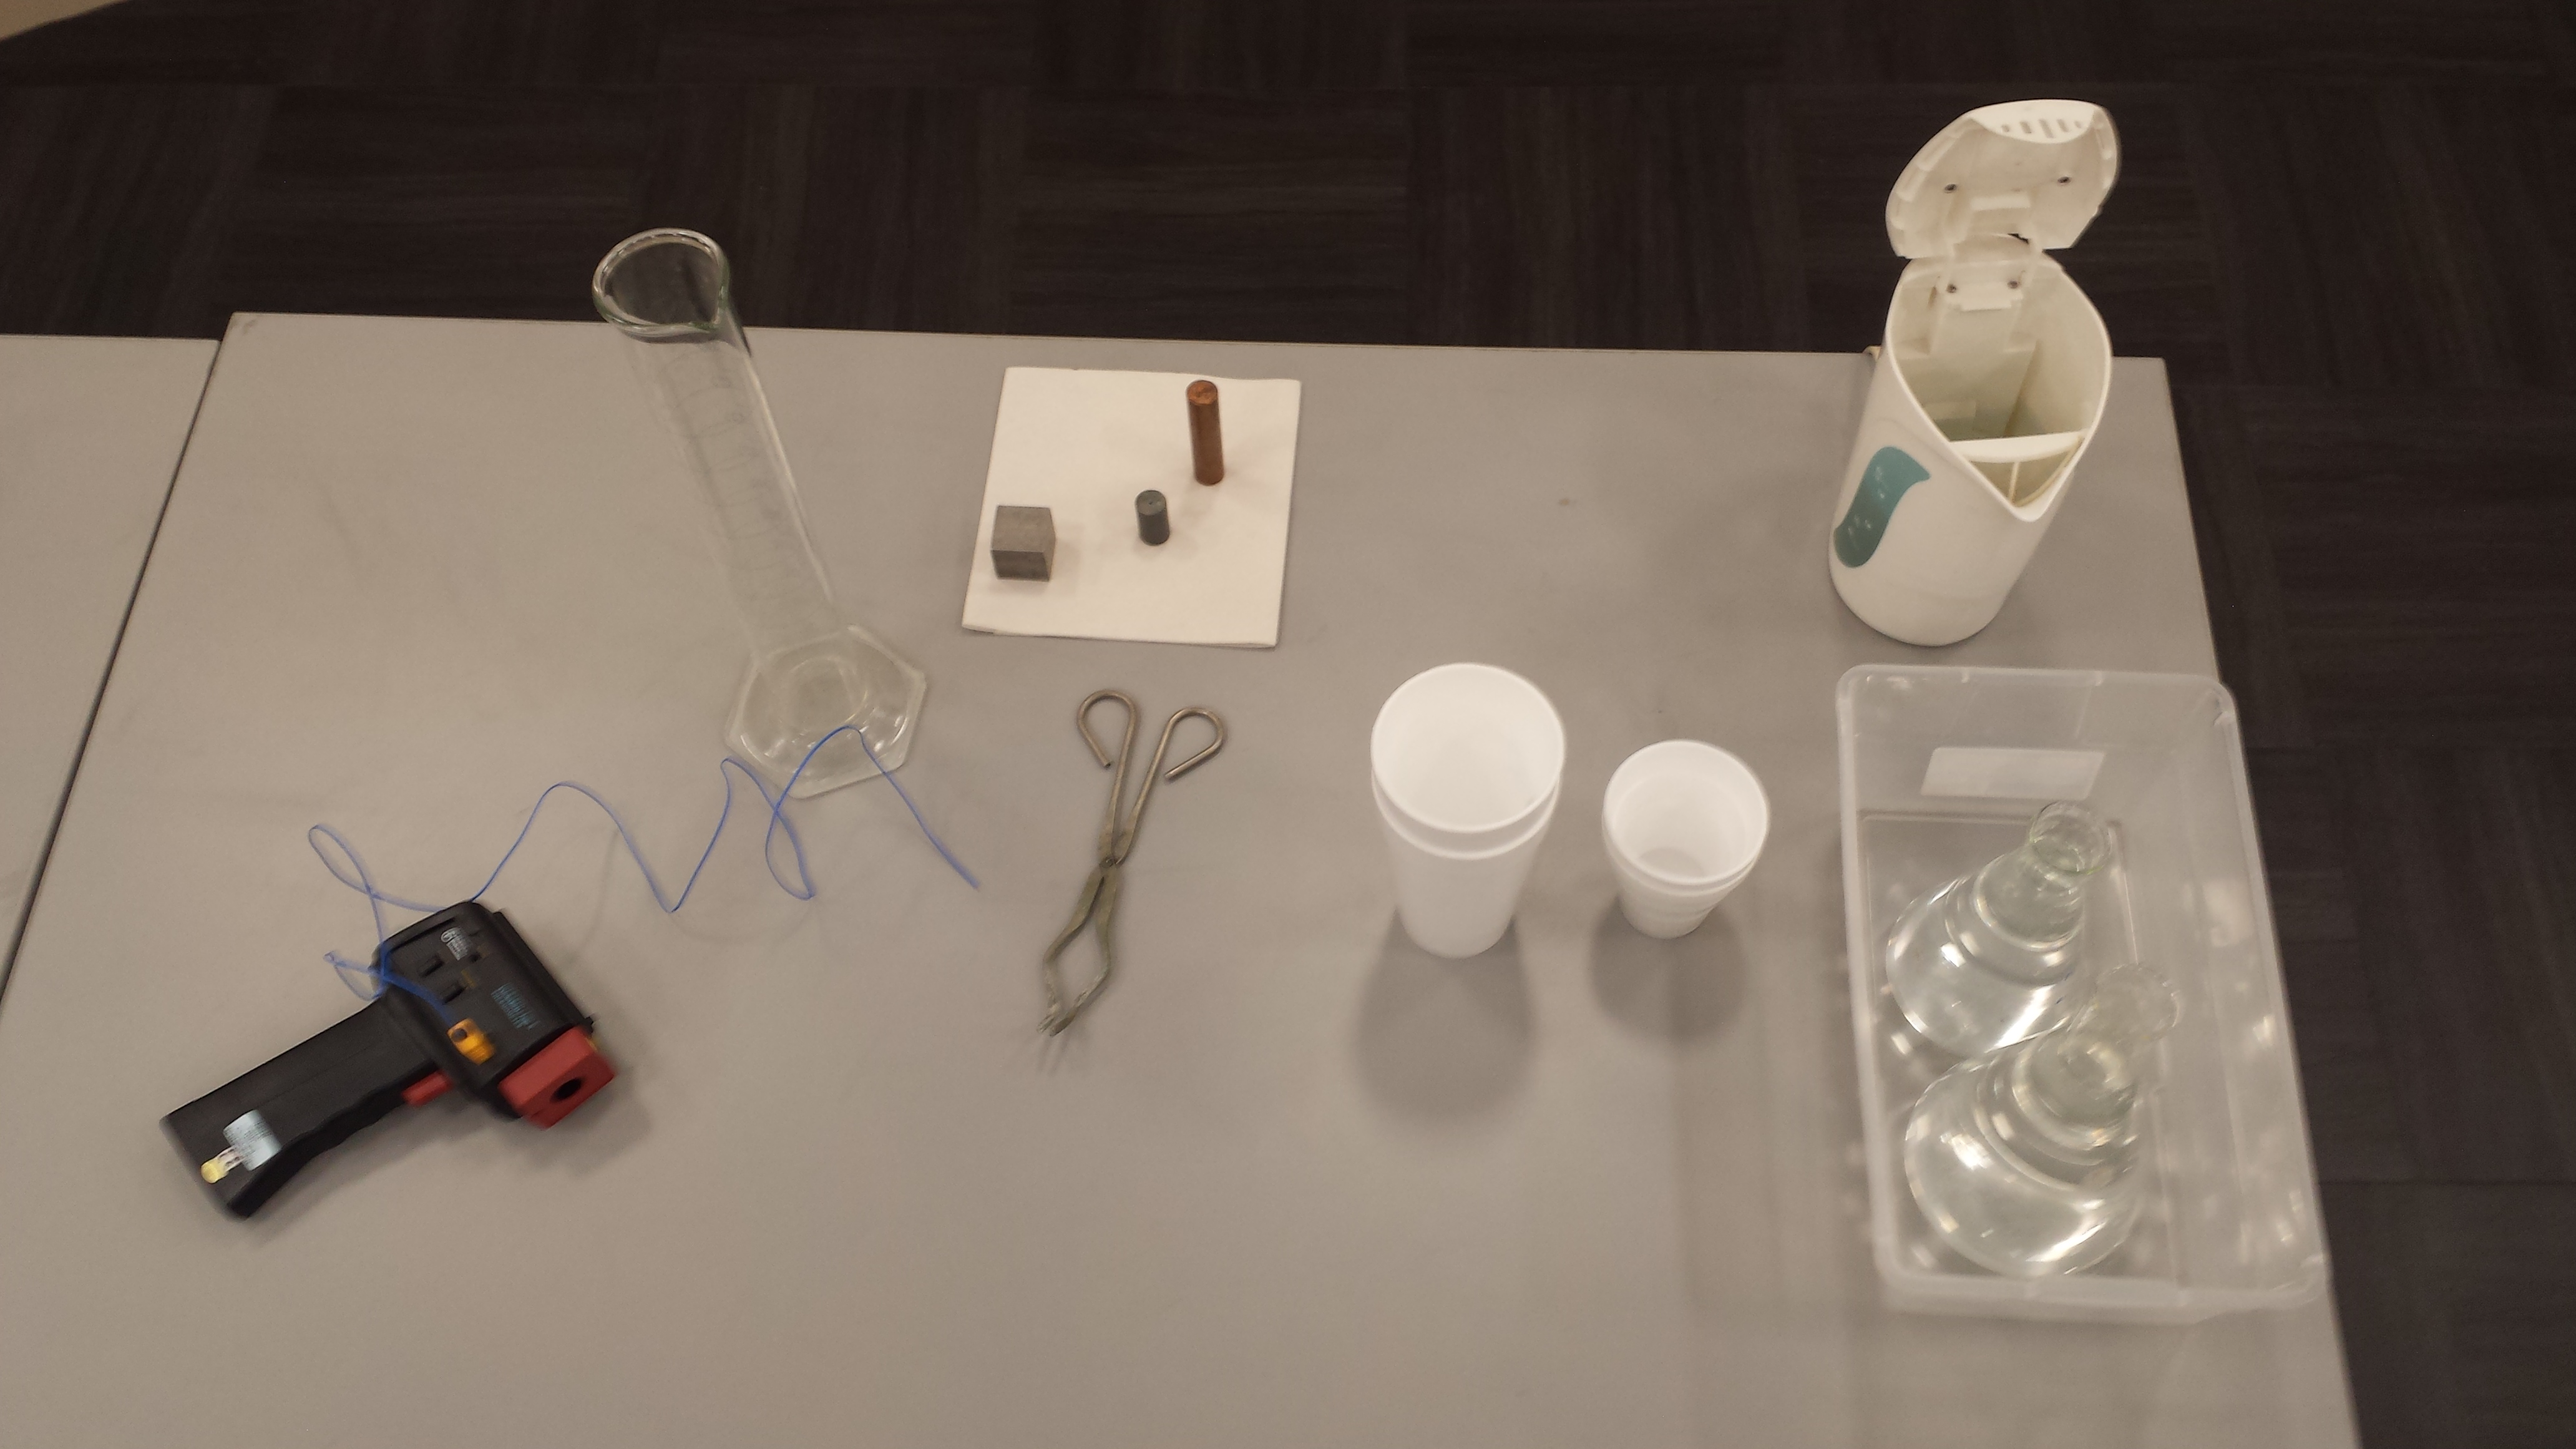
\includegraphics[width=0.4\textwidth]{pic} % Include the image placeholder.png
\caption{Experimental materials}
\end{center}
\end{figure}

\newpage



%----------------------------------------------------------------------------------------
%	BIBLIOGRAPHY
%----------------------------------------------------------------------------------------

\bibliographystyle{apalike}

\bibliography{sample}

%----------------------------------------------------------------------------------------


\end{document}